%!TEX root = ../../Master.tex
\section{Organisation}

Det følgende afsnit vil analysere de kontekstuelle forhold for det, som beskrives af Laudon \& Laudon som \enquote{organisation}. Dette vil også inkludere en interessent analyse, i overensstemmelse med rapportens format. Valg af elementer i kategorien \enquote{organisation}, sker på baggrund af en brainstorm omkring hvilke organisationer der vil blive berørt, samt ud fra de fortaget interviews. Dette afsnit er delvist forbundet med menneske afsnittet, og bør læses i forlængelse af hinanden, for at opnå en samlet forståelse.

\subsection{Foreninger} % (fold)
\label{sub:Foreninger}

\subsubsection{Dansk Sejlunion} % (fold)
\label{ssub:Dansk Sejlunion}

Der eksisterer mange foreninger for både/sejlklubber i Danmark. En af de største unioner er Dansk Sejlunion, som er et specialforbund under Dansk Idræts Forbund. DS optager klubber i alle former for sejlads som medlemmer. DS har en kollektiv forsikring som alle 273 medlemsklubber automatisk er medlem af, samt andre fordele for medlemsklubberne. Dette inkluderer rabattter på Falck søsikkerhedspakken, sejlershoppen.dk og Mols-linien, samt juridisk rådgivning \cite{ds_optagelse,ds_fordele}.

Idet DS har så mange medlemsklubber, er denne forening relevant i forhold til at sælge et eventuelt IT-system til sejlklubber i Danmark. DS tilbyder på deres hjemmeside en liste over leverandører af administrationsløsninger til deres medlemmer. Et IT-system på denne liste, vil uden tvivl opnå højere synlighed for eventuelle kunder.\cite{DanskSejlunionKlubAdmin}

% subsubsection Dansk Sejlunion (end)

\subsubsection{Aalborg/Nørresundby Fritidshavn}

En anden vigtig forening, er den lokale paraplyorganisation Aalborg/Nørresundby Fritidshavn bosiddende i Aalborg.

Der er 4 store lystbådehavne i Aalborg by:
\begin{itemize}[noitemsep]
    \item Marina Fjordpark
    \item Skudehavnen - lystbådehavnsafsnit
    \item Vestre Baadehavn - lystbådehavnsafsnit
    \item Nordre Baadehavn
\end{itemize}

I Aalborg er det kommunen der ejer alle havnene. ANF, en paraplyorganisation for sejlklubsforeninger i Aalborg/Nørresundby, får lov til at bruge disse havne i mod at havnene bliver vedligeholdt. Foreningerne i ANF kan så leje havnene af ANF. Der er typisk en bådklub pr. havn. Nogle havne benyttes også af mindre klubber som kajakklubber eller søspejdere  \cite{int_vb_sl}.

ANF er en paraplyorganisation for følgende sejlklubber \cite{anf_havnereglement}. Se \cref{fig:anf_overblik}.
\begin{itemize}[noitemsep]
	\item Aalborg Sejlklub
	\item Fiskerklyngen
	\item Vestre Baadelaug
	\item Sejlklubben Limfjorden
	\item Nørresundby Sejlklub
\end{itemize}
 
ANF forestår forhandlinger på vegne af organisationens sejlklubber. En fælles brugsaftale af de fire havne, kan derved indgås med havneejer, Aalborg Kommune.

ANF's indtægter består af bådpladsafgifter, som medlemsklubberne skal betale for brug af de tilknyttede havne \cite{anf_budget_2013}. Det er op til de enkle klubber at fordele deres pladser ud til medlemmerne. ANF forpligter sig til vedligeholdelse af havnene tilknyttet foreningen, herunder hovedistandsættelser samt udføring af nyanlæg. \cite{anf_brugsaftale_2012}.

\begin{figure}
  \centering
  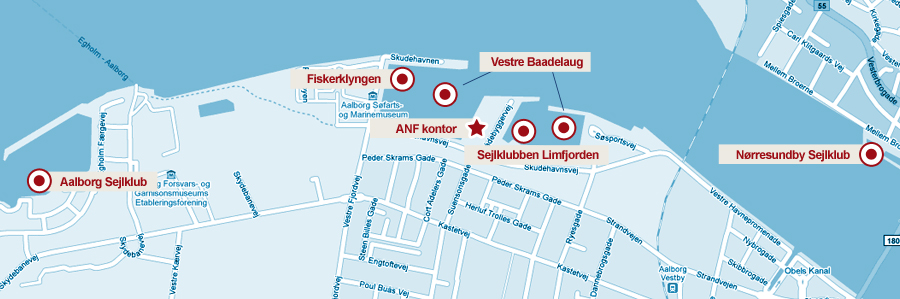
\includegraphics[width=\textwidth]{anf_overblik.jpg}
 	\caption{Overblik over medlemmerne af ANF} 	\label{fig:anf_overblik}
\end{figure}

% subsection Foreninger (end)


\subsection{Bådklubber}
Her vil vi se på de bådklubber der er tilknyttet Vestre Bådehavn og Skudehavnen.

\subsubsection{Vestre Baadelaug}
Vestre Baadelaug har bådpladser i Vestre Bådehavn og Skudehavnen, som begge deles med Sejlklubben Limfjorden. I Vestre Baadelaug, fordeles disse pladser hvert år ud til medlemmerne. Inden den nye pladsfordeling bliver lavet, er det muligt at ønske en bestemt plads. Der er en masse menneskelige interesser der skal varetages når pladserne skal fordeles. Det er vigtigt for nogle medlemmer hvor de ligger. Det er ikke muligt at få en permanent plads, men kassereren sørger for at et medlem beholder sin tidligere plads når fordelingen bliver lavet. Medlemmerne betaler pr.\ kvadratmeter. Kvadratmeterne kan opgøres på forskellige måder, f.eks.\ som plads arealet eller som bådarealet. Et medlem kan kun have én bådplads, dog kan der opstå situationer hvor et medlem har mere end en båd, bl.a.\ i forbindelse med salg af en båd. Klubben har omkring 380 medlemmer \cite{int_vb_sl}.

\frnote{lidt mere om herakiret i klubben. forman/næsteformand osv.
}

\subsubsection{Sejlkubben Limfjorden}
Sejlkubben Limfjorden har omkring 150 medlemmer \cite{int_vb_sl}. Klubbens medlemmer omfatter kun personer med sejlbåde. Klubben er medlem af Dansk Sejlunion.

%% Fr: det skal vi nok ikke havde med
%\subsubsection{Aalborg Sejlklub}
%Aalborg Sejlkulb er en Sejlklub, der hører til i havnen Marina Fjordparken. Nørresundby Sejlklub er tilknyttet Nørresundby havn. Klubben er medlem af Danske Tursejlere \cite{norresundby_sejlklub}.

\subsection{Regler og love}
Transportministeriet har i 2002 udgivet en bekendtgørelse om standardreglement for lystbådehavne \cite{standardreglement}. I denne er der regler om hvordan medlemmer, samt gæster skal opføre sig når de befinder sig i en havn. De enkelte havne skal udarbejde et individuelt ordensreglement, som beskriver hvilket område det gælder for, og hvilke særlige ordensregler der skal gælde på havnen. Derudover skal det referere til bekendtgørelsen.

I standardreglementet bliver der beskrevet hvordan fartøjet skal fortøjes og hvordan der skal sejles i havne. Blandt andet står der at gæstende fartøjer skal melde deres ankomst til havnemyndigheden, og de skal flytte deres fartøj til en anden plads hvis havnemyndigheden siger det. Føreren af ethvert fartøj har også pligt til jævnligt at holde øje med sit fartøj, når det ligger i havnen. Fartøjet skal være forsvarligt fortøjret og tov skal fastgøres så de ikke klapper mod masten. I reglementet er der regler for optagning, reparation, brændstof og forskellige miljøbestemmelser.

Ifølge standardreglementet er det havnemyndigheden der står for at holde orden på et havneområdet. Enhver som befinder sig på havneområdet skal overholde havnemyndigheddens anvisninger. Politiet og andre myndigheder skal stadigvæk udføre deres opgaver inden for deres lovgivningsmæssige regler. De fleste regler i standartreglementer kan omgås hvis der gives tilladelse fra havnemyndigheden. Hvis en regel ikke bliver overholdt kan havnemyndigheden flytte den pågældende båd for ejerens regning.


\subsection{Aalborg Kommune}
Aalborg Kommune er kendt i landet som en uddannelsesby på grund af Aalborg Universitet og Aalborg Kommune ligger stor vægt på at byen skal være attraktiv for studerende, ved at prioritere ungdomsboliger og universitets velvære højt. \cite{udd-strat-aalborg} Aalborg by er kendt for dets store karnevald, Aalborg Zoo, Aalborg Kongres \& Kultur Center og Vor Frue Kirke. \cite{AalborgAttraktioner} Aalborg Kommune forsøger at få et mere "levende og kreativt kulturmiljø" \cite{AalborgSatserPåKultur}, og de har sat 310 mio kroner af til at forbedre Aalborgs kulturliv. Heriblandt inbdgår Aalborgs rige havnemiljø, med bådklubber, besøgende krystogter og havnefronten. \cite{AalborgHavnefront} For at opnå et levende og kreativt kulturmiljø er Aalborg Kommune interesseret i bådklubbernes velvære og funktionalitet.
